\chapter{Etude de cas : Les Smart Cities}



%%%%%%%%%%%%%%%%%%%%%%%%%%%%%%%%%%%%%%%%%%%%%%%%%%%%%%%%%%%%%
%% 
%%%%%%%%%%%%%%%%%%%%%%%%%%%%%%%%%%%%%%%%%%%%%%%%%%%%%%%%%%%%%
\section{Introduction}
Le concept de Smart City est fondé sur les intérêts qu'auraient les métropoles à utiliser les technologies d'information et de communication pour y booster l'efficacité des différents flux et minimiser les pollutions. En effet, l'objectif est de remplacer les prises de décision politiques par des choix basés sur des masses de données récoltées par un grand nombre de capteurs situés partout dans la ville. Cela nécessite l'utilisation d'un modèle 3D poussé : les informations obtenues en temps réel par les capteurs ne prennent un sens que lorsqu'ils sont mis en relation et en contexte. En outre, certaines études ne peuvent en pratique se faire qu'avec un modele 3D. Par exemple l'étude des écoulement et drainage des eaux.

%A faire : 
%- Introduire ce qu'est une smart city et comment ça peut être l'évolution de notre mode dans les prochaines années

%\section{Les enjeux}
%- parler de l'enjeu d'avoir une représentation 3D précise de celles ci (aller voir sur internet, exemples : calcul des flux pour l'optimisation, gestion thermique, gestion des risques (criminels  -> camera), réseau centralisé des risques...)
%- Expliquer que c'est un domaine d'avenir : mettre des budgets allouer ou des papier sur là ou on va
%
% * <anatole.maurer@telecom-sudparis.eu> 22:42:07 10 Feb 2022 UTC+0100:
% du coup tout ca c'est deja un peu dans lintro ...
%Lisez ce papier https://www.gim-international.com/magazines/gim-international-september-october-2018.pdf vous verez toute les Utilisation possibles.


\section{Modélisation 3D}

La première étape pour obtenir une version jumelle d'une ville dans le monde 3D est d'obtenir sa copie. En effet, il nous en faut une représentation 3D. Cependant, il est nécessaire d'avoir une représentation particulière : il nous faut une représentation qui puisse être ensuite utilisée de façon complexe. Il nous faut donc une version enrichie de la ville, une version qui ne soit pas juste de la donnée géométrique mais qui puisse contenir les interactions de chaque composant les uns avec les autres (par exemple les feux de circulation avec la gestion de flux...)
Nous allons étudier comment obtenir cette représentation 3D en plusieurs étapes : il faut tout d'abord en obtenir une version 3D sous forme de nuage de points, puis la convertir en mesh, avant d'intégrer cette vision dans un moteur de calcul et si possible de rendu graphique.

\subsection{Acquisition 3D}
Ce rapport portant sur la notion de nuages de points et de maillages 3D, nous avons pu précédemment expliciter les différences et les liens entre ces deux représentations de données 3D. La reconstruction dans le monde virtuel d'une ville passe donc en premier lieu par une acquisition sous forme de nuage de points denses à plusieurs niveaux des données géométriques de la ville. En effet, comme nous avons pu le voir, les relevés laser permettent une acquisition simple des nuages de points et avec une grande précision sur de longues distances.
Dans la plupart des cas, la collecte est faite à deux échelles : des scanners terrestre et aérien sont utilisés. De même une combinaison de méthodes devra être utilisée; dans notre cas le plus souvent on retrouve la photogrammétrie et les scanners LiDAR.

\subsubsection{Scan au niveau du sol}
La collecte des données 3D au niveau du sol se fait très souvent à l'aide de scanner LiDAR, leur grande précision et  leur capacité de scanner rapidedement permet une plus grande flexibilité. Pour ce faire il est nécessaire d'utiliser des algorithmes de SLAM (Simultaneous Localisation And Mapping) \cite{LOAM} qui permettent de suivre le capteur et de projeter les nuages de points obtenus dans une carte 3D globale qui peut ensuite être combinée avec d'autres cartes pour obtenir la ville :

Pour ce faire il nous faut un rig avec un LiDAR et des cameras RVB pour obtenir un nuage de points colorés :
\begin{figure}[h]
    \centering
    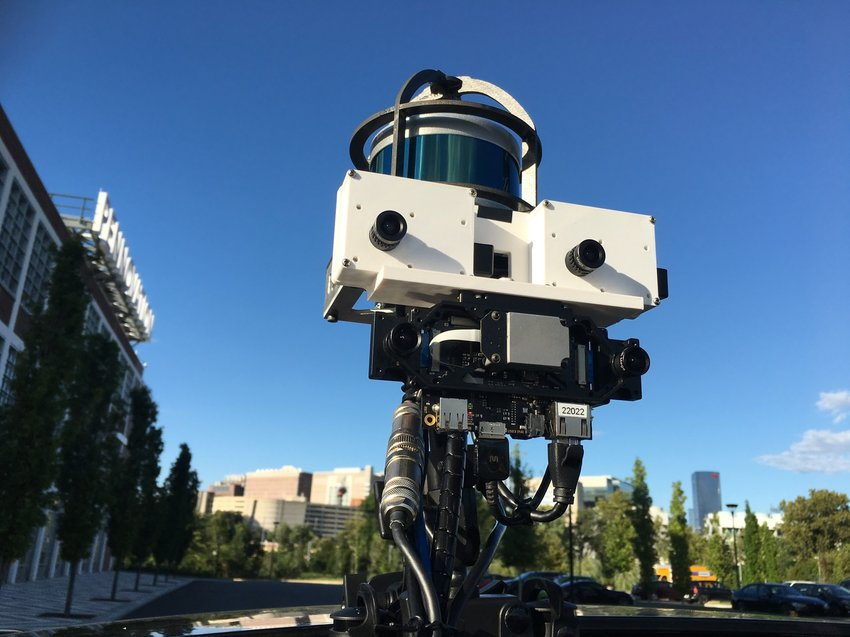
\includegraphics[width=0.50\textwidth]{rig}
    \caption{Exemple de rig de scan au sol}
    \label{fig:solrig}
\end{figure}
\FloatBarrier

Puis l'utilisation d'un algorithme de SLAM pour enregistrer le nuage de points. On peut alors, pour obtenir une carte avec une position absolue, combiner des données GPS et inertielles dans le SLAM directement :

\begin{figure}[h]
    \centering
    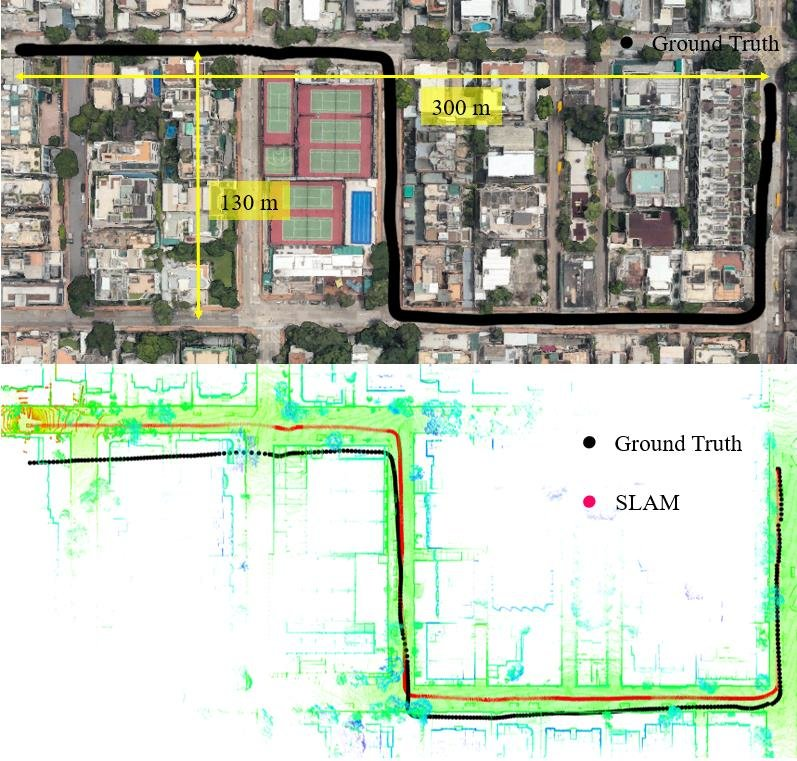
\includegraphics[width=0.50\textwidth]{slam}
    \caption{Chemin du capteur retrouvé par l'algo de SLAM}
    \label{fig:solrig}
\end{figure}
\FloatBarrier

\newpage

Finalement après avoir scanné la ville, on obtient un nuage de points au niveau du sol précis de celle ci :
\begin{figure}[h]
    \centering
    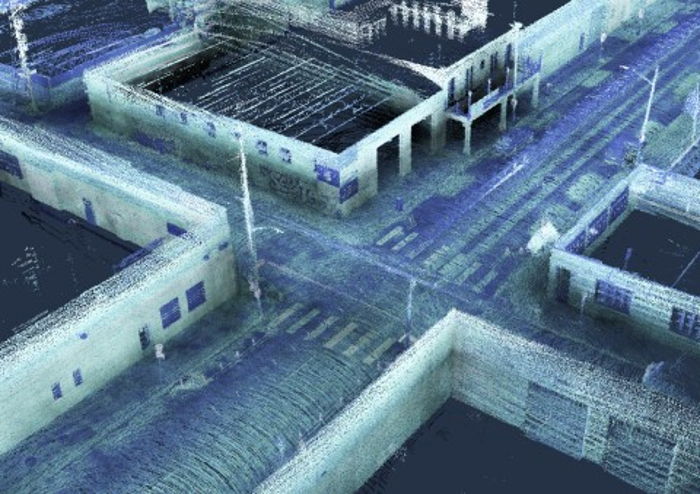
\includegraphics[width=0.50\textwidth]{ground}
    \caption{Vision en nuage de points au niveau du sol}
    \label{fig:sol}
\end{figure}
\FloatBarrier

\subsubsection{Cartographie 3D aérienne}

Il faut maintenant obtenir une vue plus globale de la ville pour, une fois combinée avec notre scan au sol, obtenir l'ensmeblede la ville.
Pour ce faire nous allons combiner les méthodes de photogrammétrie et de scan laser à bord d'un avion : le scan laser permet d'avoir avec précision les distance, tandis que le scan photogrammétrique permet d'avoir  la couleur associée ainsi que certains détails.
\begin{figure}[h]
    \centering
    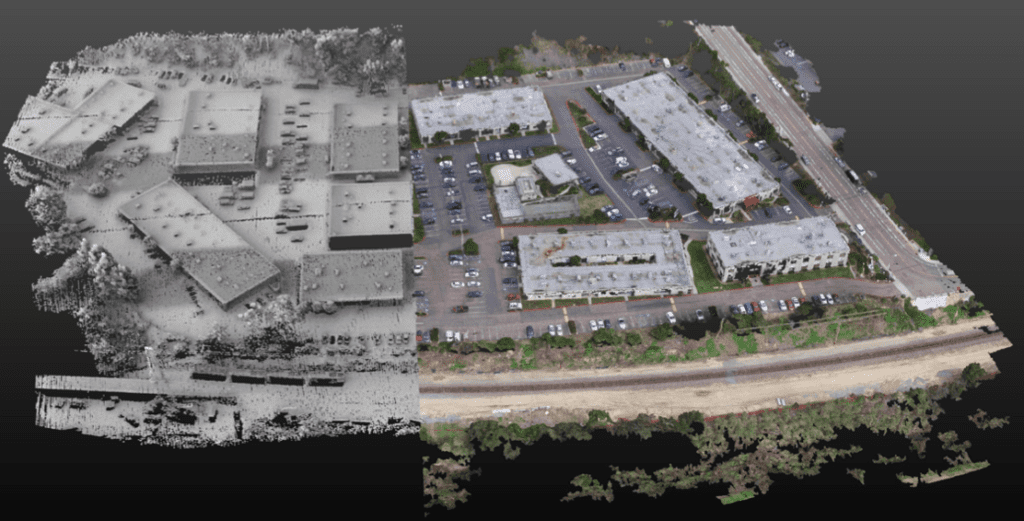
\includegraphics[width=0.8\textwidth]{lidarPhoto}
    \caption{Fusion des données LiDAR et Photogrammétriques}
    \label{fig:sol}
\end{figure}
\FloatBarrier

\newpage

Une fois ces deux types d'acquisitions terminées, il faut ensuite combiner les nuages de points obtenus pour récupérer une carte de nuage de points dense.
\newline

\begin{figure}[h]
    \centering
    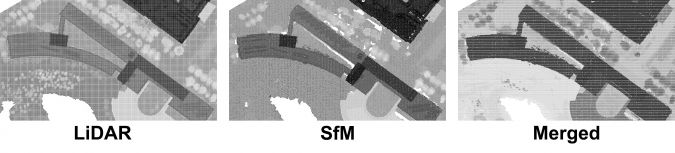
\includegraphics[width=0.8\textwidth]{merge}
    \caption{Combinaison des deux cartes : sol + aérien}
    \label{fig:sol}
\end{figure}
\FloatBarrier
C'est à partir de ce nuage de points dense que nous travaillerons dans la suite.
\begin{figure}[h]
    \centering
    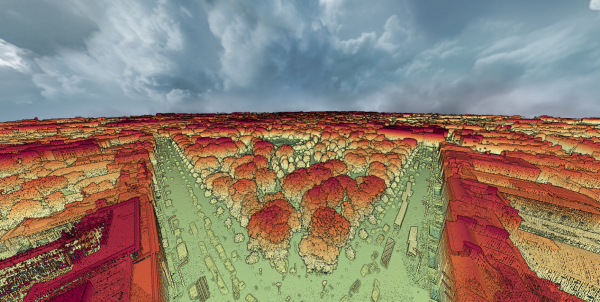
\includegraphics[width=0.8\textwidth]{cityscan}
    \caption{Résultat final de la ville en nuage de points}
    \label{fig:sol}
\end{figure}
\FloatBarrier

\paragraph{Pour aller plus loin} Nous n'avons ici fait que présenter la surface du sujet. Cependant, il y a beaucoup de recherche dans ce domaine; Que ce soit au niveau du SLAM : comment arriver à faire des slam de très grande envergure en limitant l'erreur \cite{slamLargeScale} ou comment réaliser des slam avec différents types de données (GPS, IMU...), mais aussi sur de la photogrammétrie de grandes étendues \cite{LargeScale}. Tout comme la gestion des nuages de points, la fusion de nuages denses est un champ actif de recherche. Cependant, la présentation de tous ces domaines sortirait du cadre de ce document.

\subsection{Transformation en maillage 3D et format spécialisé}

Une fois le nuage de points obtenu, il est maintenant question de le transformer en maillages 3D qui, si possible, pourront être utilisés par la suite dans une application spécialisée pour associer à chaque catégorie d'intérêt un traitement spécifique : centrale électrique, résidences, immeubles...
\newline
Pour réaliser cette différenciation nous allons devoir classifier le nuage de points. La recherche dans ce domaine est la aussi très dynamique. Pour ce faire, des méthodes de classification algorithmique seront généralement utilisées : Support Vector Machine, K nearest search ou random forest. Cependant, les méthodes par machine learning deviennent de plus en plus concluantes. On peut par exemple citer : kpconv net \cite{thomas2019KPConv} ou encore pointnet++ \cite{qi2017pointnet}.
\newline
Grâce à ces différentes méthodes, on peut alors segmenter notre nuage de points :
\begin{figure}[h]
    \centering
    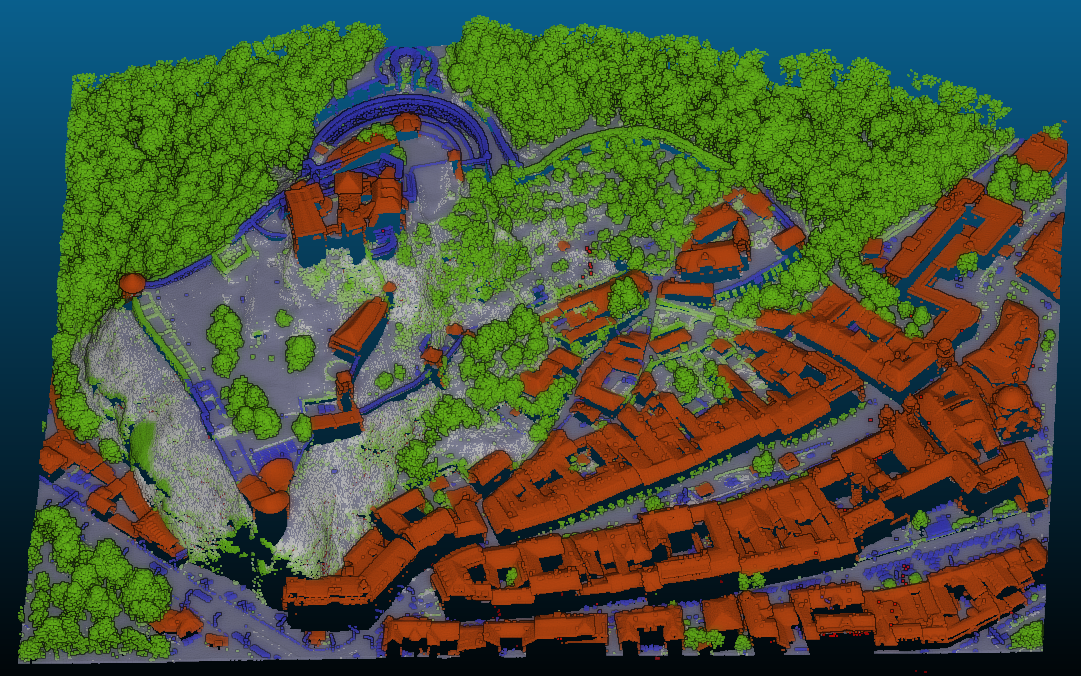
\includegraphics[width=0.65\textwidth]{clas}
    \caption{Nuages de points classifiés}
    \label{fig:sol}
\end{figure}
\FloatBarrier

A partir de ce nuage classifié, il vient alors la reconstruction de modèle sous forme de maillage 3D. Ici aussi, en fonction du type de donnée que l'on veut récupérer à la fin la reconstruction ne sera pas la même. Par exemple les bâtiment devront être convertis sous le format de données BIM (Building information modeling), le sol sous forme DST (Digital Surface Terrain), etc. Cette étape sera ici considérée comme une étape de conversion du nuage de points en maillages 3D. En effet, comme nous l'avons vu précédemment, pour permettre un rendu visuel optimisé, pour le traitement et l'analyse de ces données, l'utilisation de maillages 3D est nécessaire (impossible d'obtenir des résultats concluant sous forme de nuages de points).
Nous obtenons alors un modèle 3D sous forme de maillages 3D très précis de la ville :

\begin{figure}[h]
    \centering
    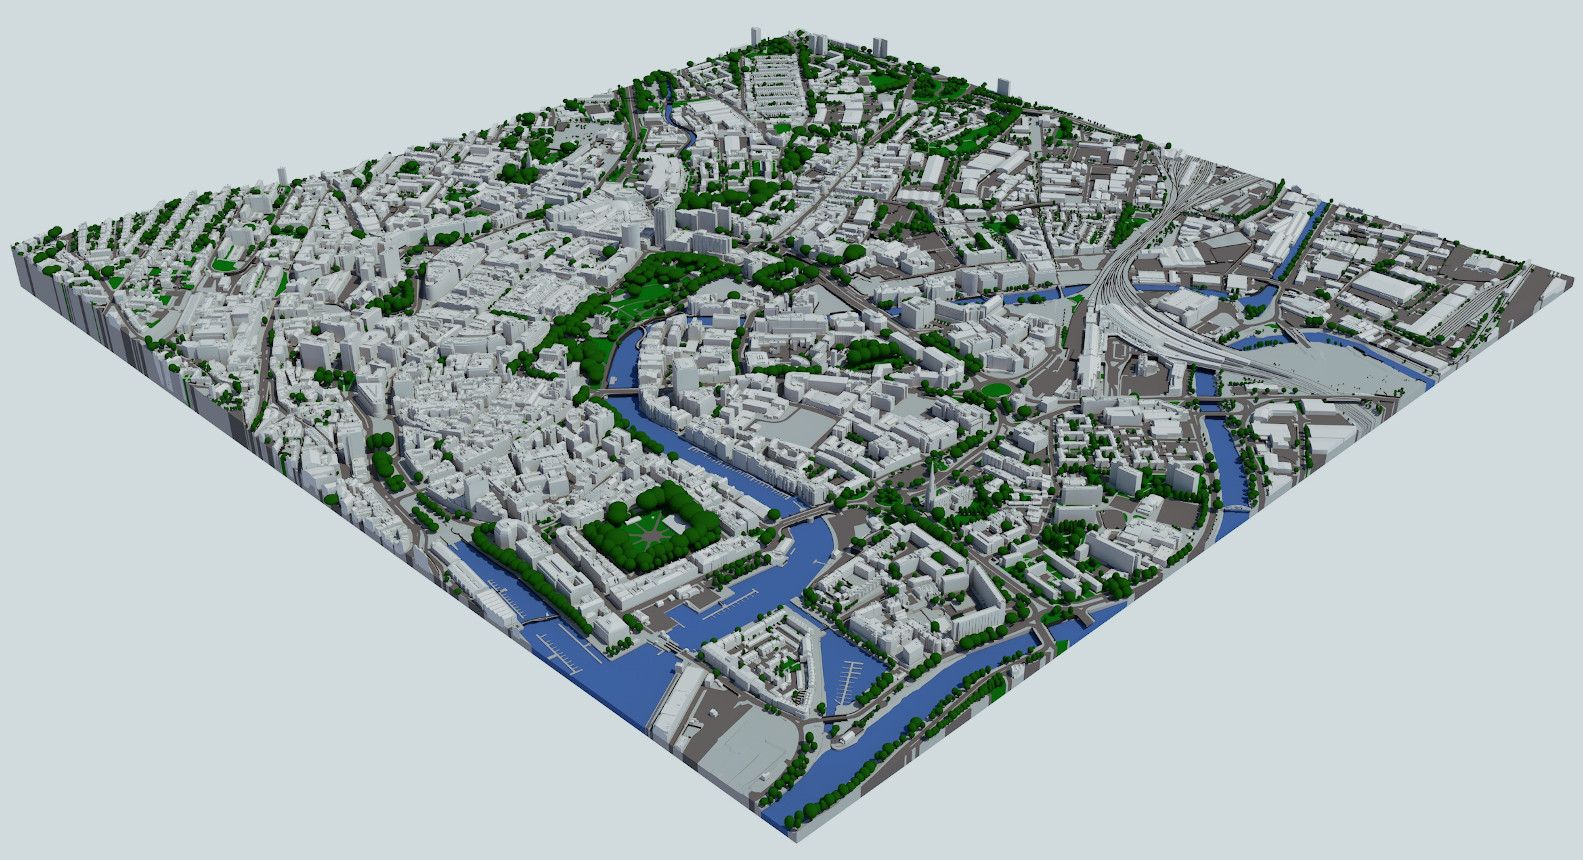
\includegraphics[width=0.65\textwidth]{globalmap}
    \caption{Jumelle virtuelle de notre ville}
    \label{fig:sol}
\end{figure}
\FloatBarrier

\section{Utilisation de la donnée 3D}

Une fois les données traitées et la ville virtuelle jumelle obtenue, nous pouvons maintenant l'utiliser pour visualiser, analyser ou simuler ses états : nous avons construit une représentation globale de la ville.

\subsection{Simulation}
La ville jumelle obtenue peut être utilisée dans le cadre de simulation grandeur nature avec une très grande complexité. Aujourd'hui les besoins de simulation sont de plus en plus grands : simulation des flux de personnes, des flux d'air sur les bâtiments, de l'eau, des voitures... Tout ceci est permis de par le fait que la ville virtuelle jumelle est une copie presque parfaite. De même pour le monitoring en temps réel : cette copie virtuelle peut être utilisée.

\begin{figure}[h]
    \centering
    \subfloat[ Simulation des flux d'air]{{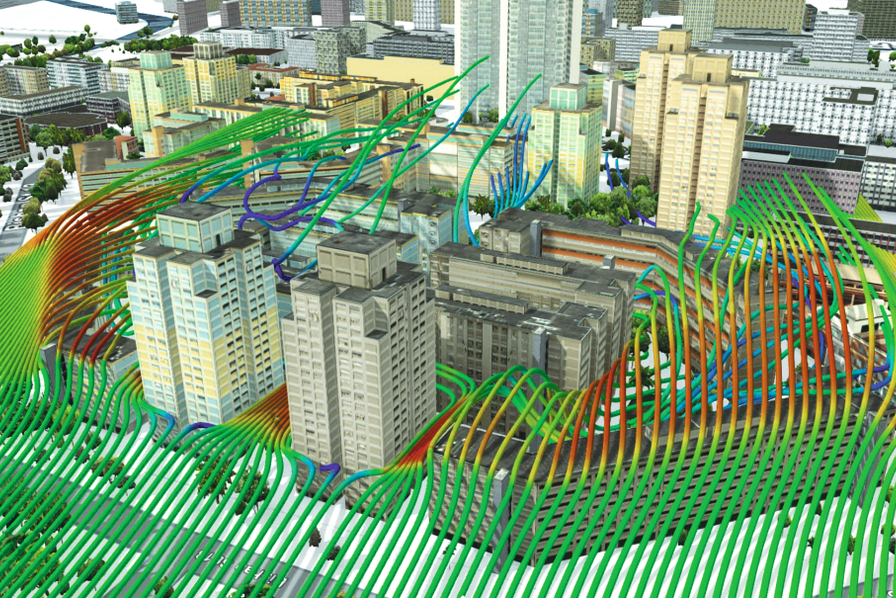
\includegraphics[width=7cm]{simmm} }}
    \qquad
    \subfloat[ Simulation de pertes thermiques]{{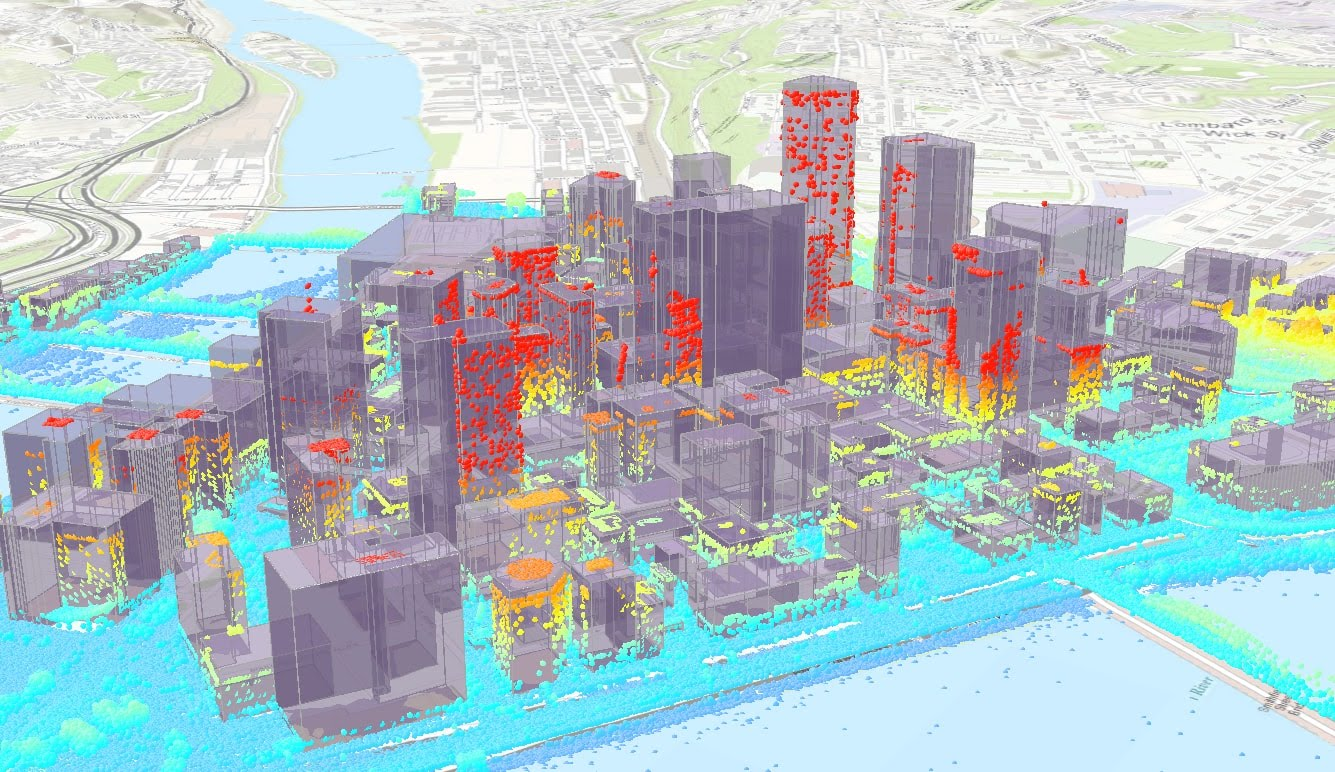
\includegraphics[width=7cm]{sim2} }}
    \caption{Utilisation de la copie virtuelle pour la simulation}
    \label{fig:Ud}
\end{figure}
\FloatBarrier


\subsection{Visualisation}
Nous avons ainsi la possibilité de l'implémenter dans un moteur graphique temps réel pour visualiser la ville et ses différents états ou évolutions (par exemple de travaux) de façon graphique et en réalité virtuelle. Certain moteurs graphiques sont spécialisés dans ce domaine, ici nous présentons Unigine :

\begin{figure}[h]
    \centering
    \subfloat[ Vision d'une ville 1]{{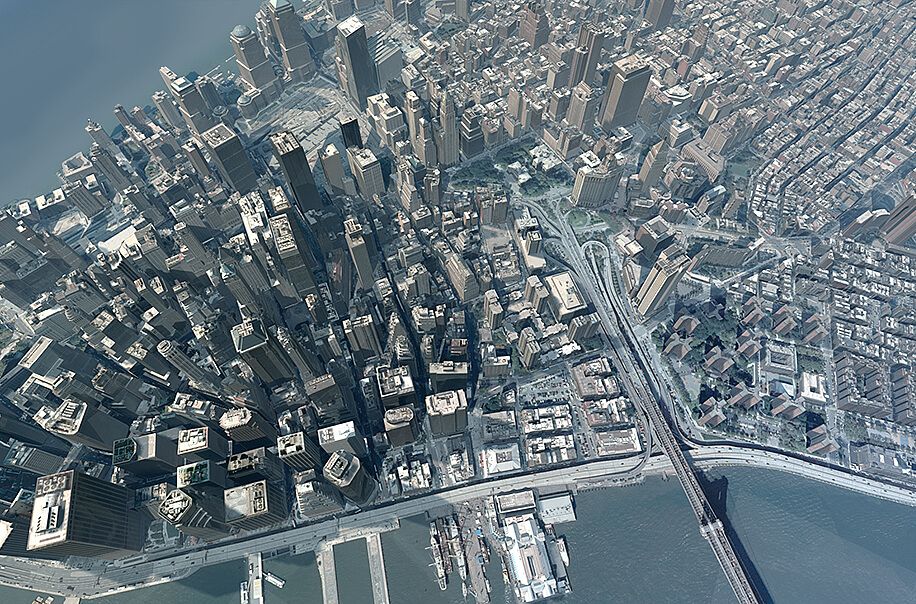
\includegraphics[width=7cm]{U1} }}
    \qquad
    \subfloat[ Vision d'une ville 1]{{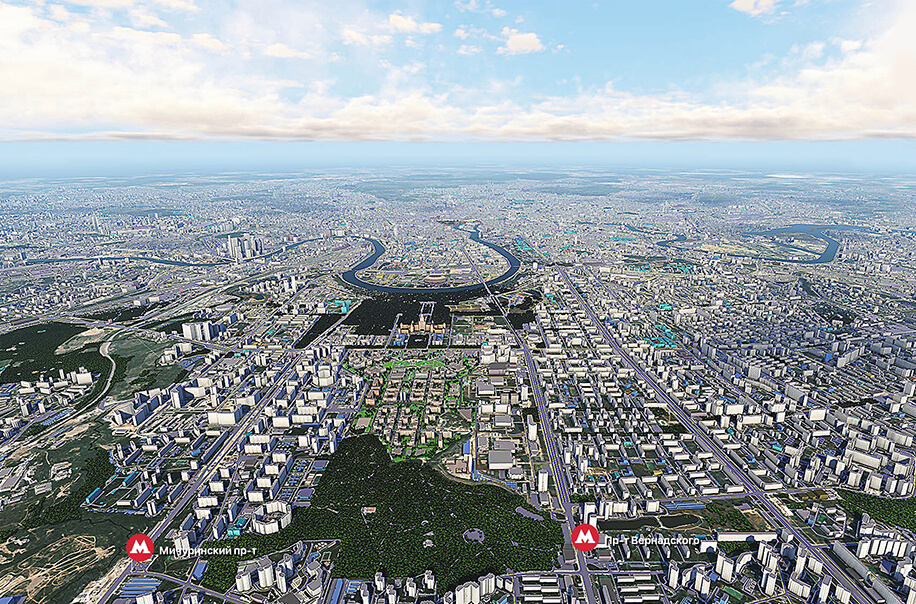
\includegraphics[width=7cm]{U2} }}
    \caption{Moteur de rendu Unigine en mode présentation}
    \label{fig:Ud}
\end{figure}
\FloatBarrier

\begin{figure}[h]
    \centering
    \subfloat[ Simulation d'une centrale]{{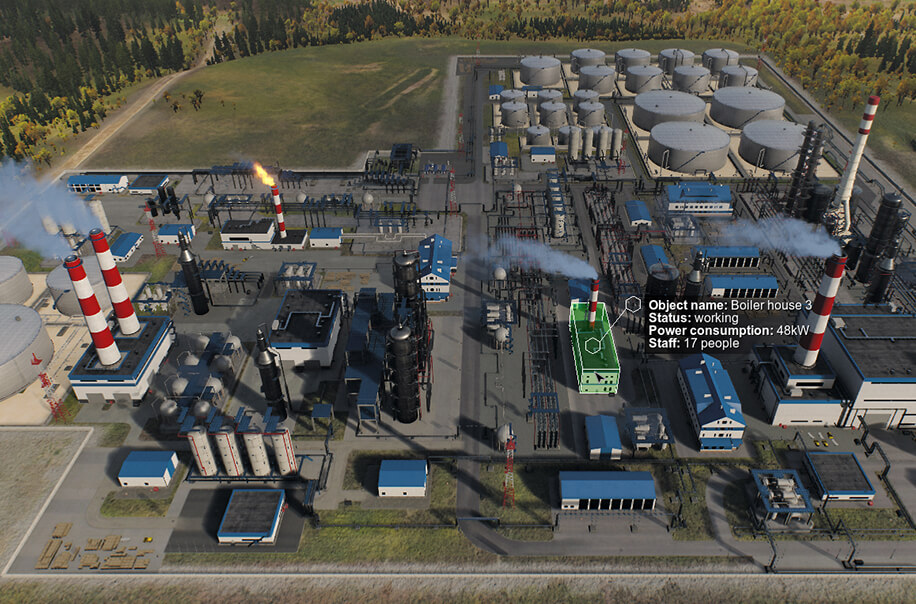
\includegraphics[width=7cm]{U3} }}
    \qquad
    \subfloat[ Simulation de la circulation]{{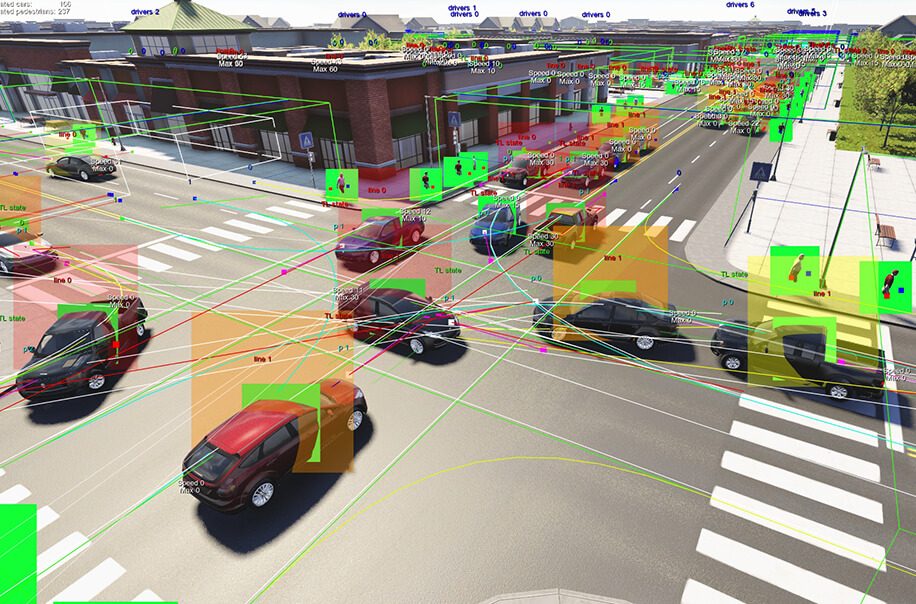
\includegraphics[width=7cm]{U4} }}
    \caption{Moteur de rendu Unigine utilisé pour la simulation}
    \label{fig:U2}
\end{figure}
\FloatBarrier


\section{Conclusion}
Pour conclure, la modélisation 3D et en particulier les maillages 3D jouent un rôle majeur pour le développement des smart cities. En effet, le développement des smart cities nécessitent une représentation 3D particulièrement fidèle à la réalité. De plus, cette représentation doit être suffisamment complexe afin de modéliser des actions et/ou événements hypothétiques. Ainsi, la représentation doit permettre de modéliser les interactions entre les différents composants de la future smart city. Par conséquent, la méthode la plus adaptée est l'acquisition d'un mesh 3d à partir d'une méthode hybride, après avoir construire au préalable un nuage de point (de préférence dense). Pour ce faire, l'usage d'un scanner Lidar est recommandée au sol en raison de sa flexibilité et efficacité d'utilisation. Cela permet en effet d'obtenir un nuage de point au sol précis. Dans un second temps, l'usage de la photogrammétrie pour associer les couleurs des objets au scan laser permettant de modéliser précisément les distances, permettront de construire un nuage de point dense de la vue aérienne de la ville. Enfin, une classification des nuages de points et différents traitements de la donnée permettent de construire un mesh 3D représentatif de la ville.
Finalement, cette représentation fidèle et complexe de la ville permet de visualiser, analyser et simuler différents événements virtuellement tels que la comparaison d'un fort ou faible afflux de personnes et/ou de véhicules, les travaux et leur évolution. Ainsi, ces simulations permises par les modélisation 3D permettront d'anticiper et réduire la consommation d'énergie, la pollution tout en améliorant l'économie et la qualité de vie des habitants grâce à la collecte et l'analyse des données virtuelles. En particulier, les risques d'inondation dans les villes côtières et/ou portuaires peuvent être réduit grâce à un croisement entre les données et propriétés de la ville, et les informations météorologiques locales.
